\documentclass[ngerman,oneside, a4letter]{article}
\usepackage[textwidth=16cm]{geometry}
\usepackage{graphicx}
\usepackage{hyperref}
\usepackage[utf8]{inputenc}
%\setcounter{chapter}{1}
\begin{document}

{\huge Python Installation}

\section{Vorbereitung}
Diese Anleitung ist für Windows ausgelegt.

\subsection{Download}
Python kann online unter \url{https://www.python.org/downloads/} heruntergeladen werden.
\\

\begin{center}
	\makebox[\textwidth]{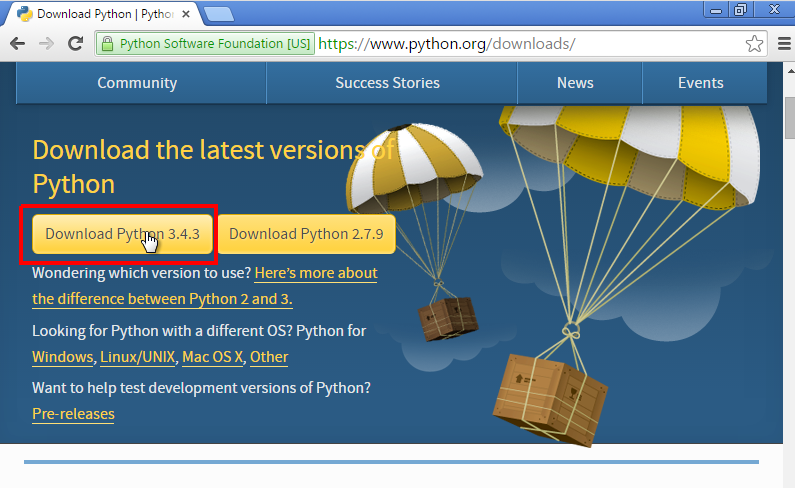
\includegraphics[width=\textwidth]{bilder/python_download}}
\end{center}
\textbf{Hinweis:} Im CoderDojo verwenden wir Python 3, deswegen ist es wichtig den Python 3-Installer herunterzuladen. Die derzeit aktuelle Version ist 3.4.3.

\clearpage

\noindent Falls der Download nicht automatisch startet, muss die korrekte Version von Hand ausgewählt werden. Hier ist die 32-bit Windowsversion zu empfehlen, sowohl für 32-bit als auch für 64-bit Systeme!
\begin{center}
	\makebox[\textwidth]{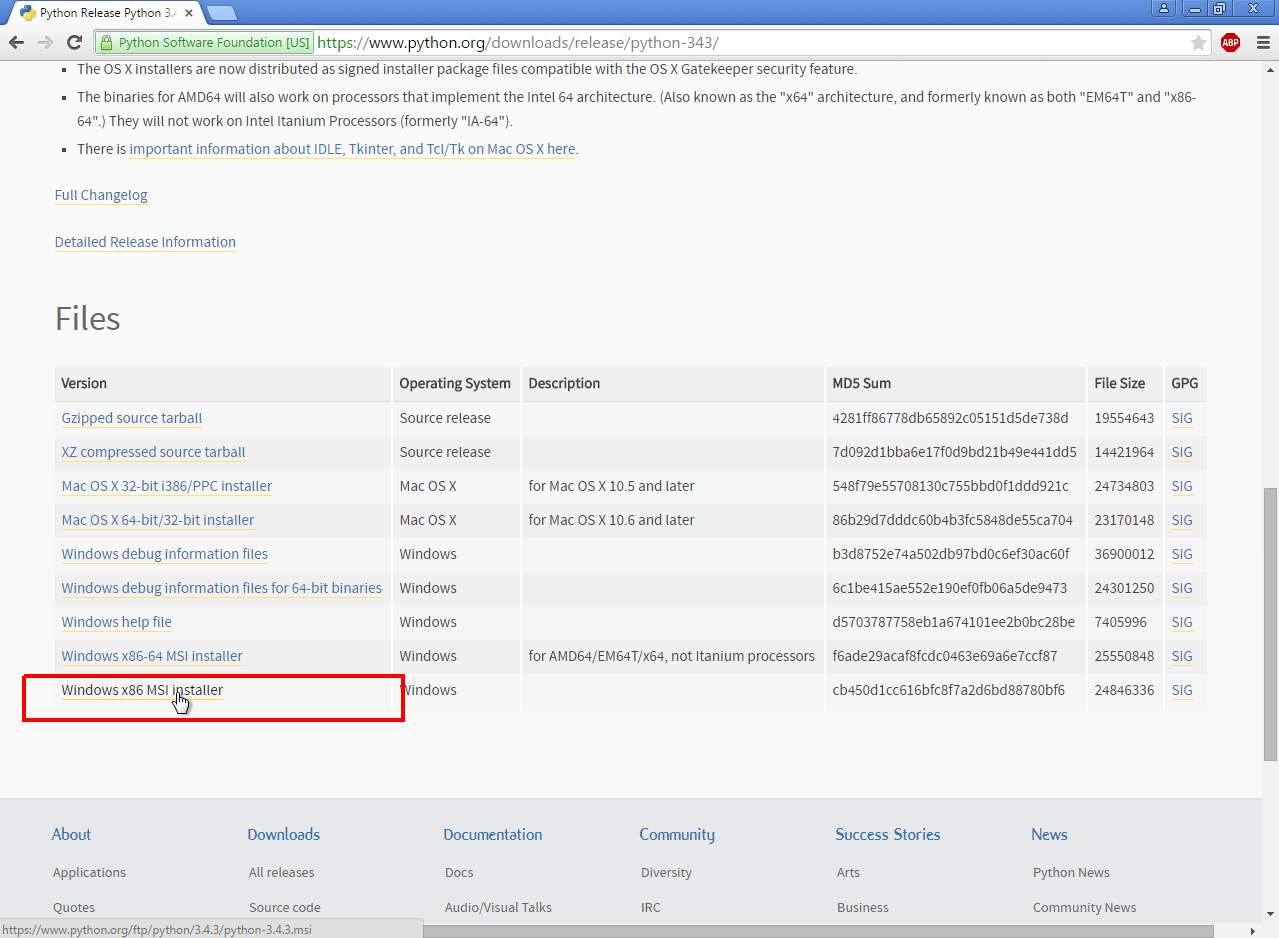
\includegraphics[width=\textwidth]{bilder/python_download_manually}}
\end{center}

\clearpage

\subsection{Installation}
Die heruntergeladene Installationsdatei kann Doppelklick gestartet werden. In den erscheinenden Fenstern auf "Weiter" und/oder "Ok" klicken um die Installation durchzuführen.
\\Die voreingestellten Werte (z.B. Installationsverzeichnis) sind gut, können aber nach Belieben geändert werden. Es muss nur Schritt \ref{path_haken_setzen} beachtet werden, um die Pfad-Variable zu setzen.

\begin{center}
	\makebox[\textwidth]{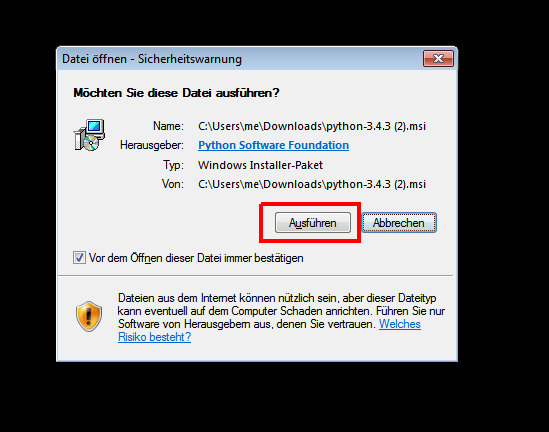
\includegraphics[width=0.9\textwidth]{bilder/install_python}}
\end{center}

\textbf{Hinweis:} Die Installation erfordert Administratorrechte.

\clearpage

\noindent Es sollte solch ein Fenster erscheienen, um die Installation zu beginnen auf 'Ok/Next' drücken.
\begin{center}
	\makebox[\textwidth]{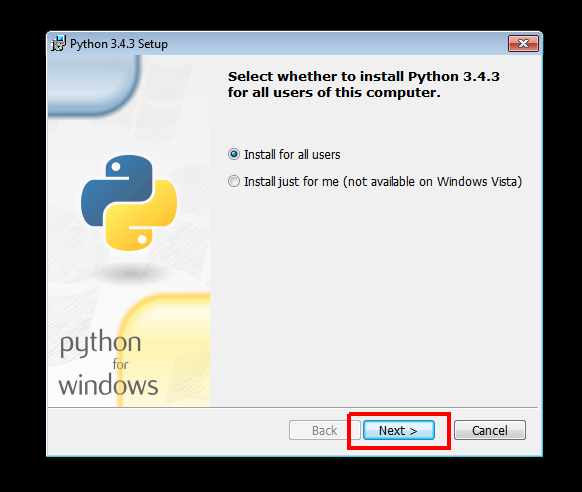
\includegraphics[width=0.9\textwidth]{bilder/install_python_start}}
\end{center}

\clearpage

\noindent\subsubsection{Pfad-Variable setzen}\label{path_haken_setzen}
\textbf{WICHTIG:} Es muss eine Einstellung angepasst werden. Wie in dem Bild zu sehen, muss die unterste Einstellungen geändert werden, damit Python zum 'System-Pfad' hinzugefügt wird. Dies ermöglicht es später Python über die Windows-Kommandozeile zu starten.
\begin{center}
	\makebox[\textwidth]{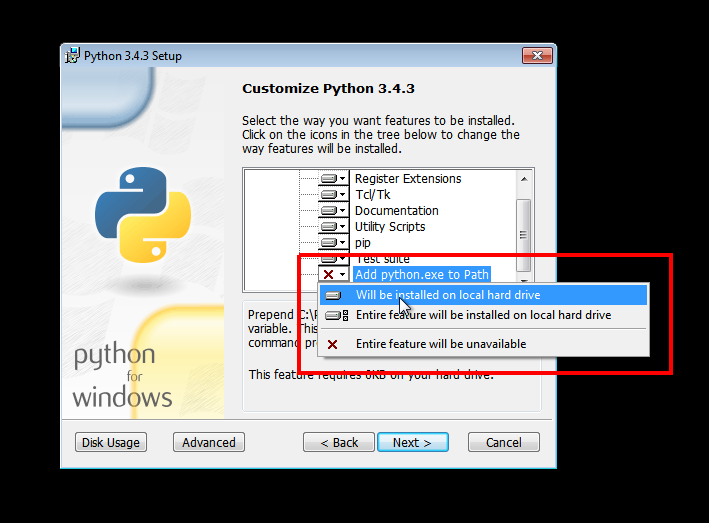
\includegraphics[width=0.9\textwidth]{bilder/install_python_path}}
\end{center}

\begin{center}
	\makebox[\textwidth]{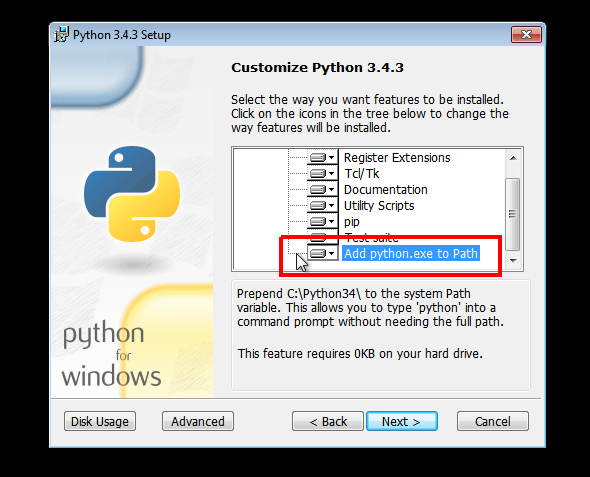
\includegraphics[width=0.9\textwidth]{bilder/install_python_path_set}}
\end{center}
Wenn die Einstellung ausgewählt ist und das Fenster an der Stelle kein rotes 'X' (vgl. obiges Bild) mehr anzeigt, kann die Installation fortgesetzt werden.

\begin{center}
	\makebox[\textwidth]{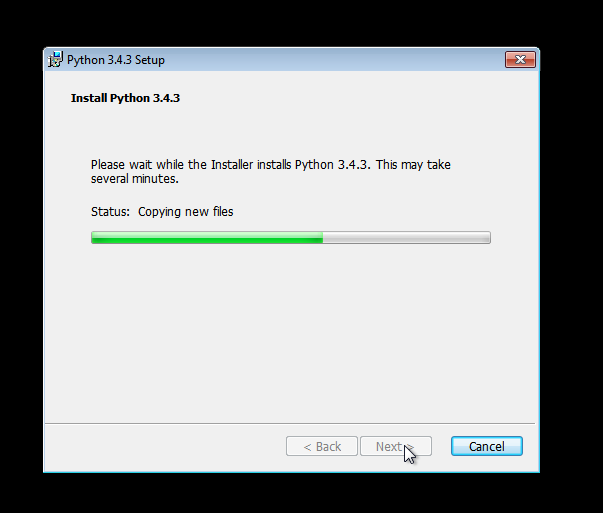
\includegraphics[width=0.9\textwidth]{bilder/python_install_progress}}
\end{center}
Die eigentliche Installation sollte nun starten, dies kann eine Weile dauern.

\begin{center}
	\makebox[\textwidth]{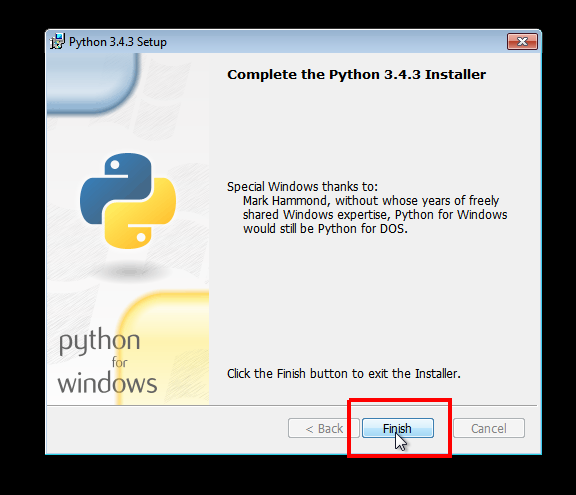
\includegraphics[width=0.9\textwidth]{bilder/python_install_finished}}
\end{center}
Ist die Installation beendet erscheint obiges Fenster. Die Installation sollte nun erfolgreich abgeschlossen sein.

\clearpage

\section{Installation überprüfen}\label{check_installation}
Ob die Installation korrekt funktioniert hat, muss jetzt noch überprüft werden. Dafür muss die Windows-Kommandozeile (CMD) geöffnet werden.
\\Diese findet man durch suchen nach 'cmd' im Windows-Suchfeld. Und startet diese durch Klick auf den gezeigten Eintrag. Ein schwarzes Fenster sollte erschienen.

\begin{center}
	\makebox[\textwidth]{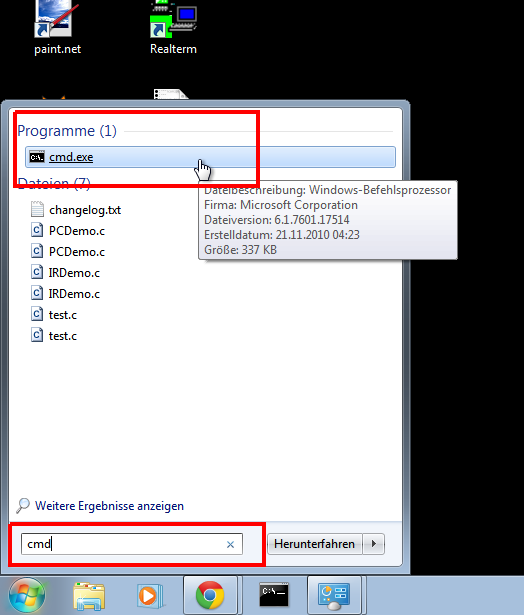
\includegraphics[width=0.8\textwidth]{bilder/cmd}}
\end{center}

\clearpage
\subsection{Python-Installation testen}
In das Kommandozeilen-Fenster tippt man nun 'python' und bestätigt durch Drücken der Enter-Taste.
\begin{center}
	\makebox[\textwidth]{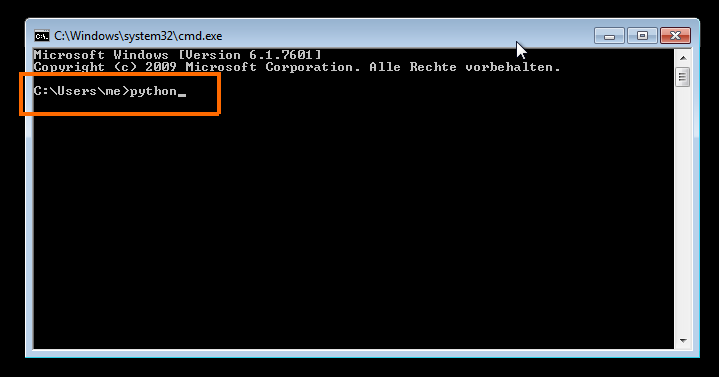
\includegraphics[width=\textwidth]{bilder/cmd_python}}
\end{center}
Hat alles geklappt sollte sich die 'Pyhton-Shell', wie in folgenden Bild öffnen.
\\
Durch tippen von 'exit()' und Bestätigen mit Enter kann diese geschlossen werden.
\begin{center}
	\makebox[\textwidth]{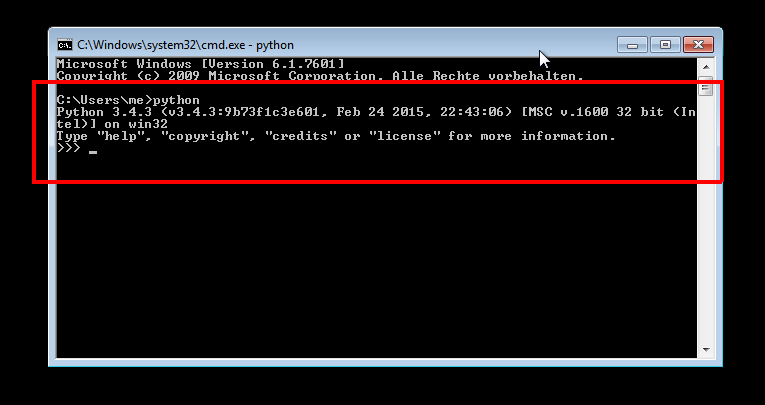
\includegraphics[width=\textwidth]{bilder/cmd_python_info}}
\end{center}

\clearpage
\subsection{Pip-Installation testen}
Mit Python 3.4 wird gleichzeitig auch 'pip' installiert. Dies ist ein sehr nützliches Werkzeug, um weitere Python-Pakete zu installieren.
\\
Dafür tippt man nun in der Kommandozeile 'pip -V'. 
\\
\\
\textbf{Wichtig:} Die zuvor geöffnete Python-Shell muss zuvor beendet (durch 'exit()') oder eine neue Kommandozeile geöffnet worden sein.
\begin{center}
	\makebox[\textwidth]{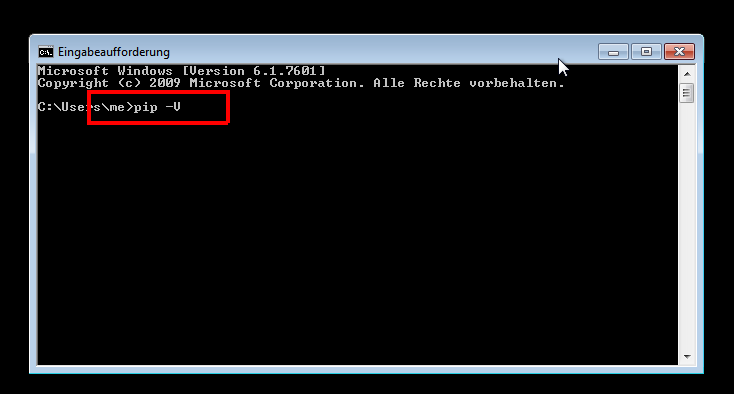
\includegraphics[width=.9\textwidth]{bilder/cmd_pip}}
\end{center}
Hat alles geklappt sollten Versionsinformationen zu 'pip' erscheinen.
\begin{center}
	\makebox[\textwidth]{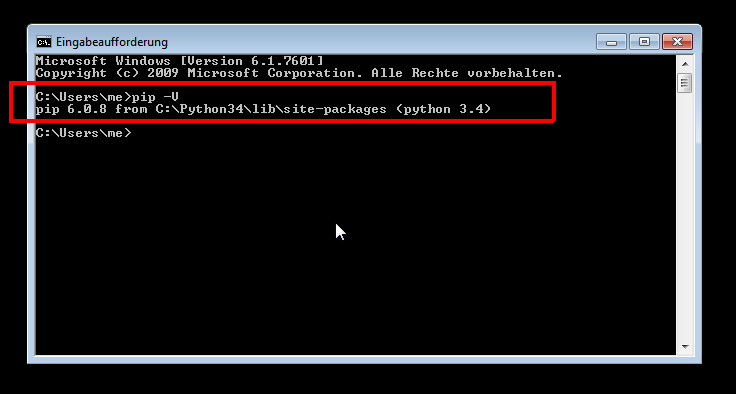
\includegraphics[width=.9\textwidth]{bilder/cmd_pip_info}}
\end{center}


Die Installation war erfolgreich! Python kann jetzt auf diesem System verwendet werden!







\clearpage
\section{Manuelles Anpassung der Pfad-Umgebungsvariablen}
\textbf{WICHTIG: } Ist die Installation erfolgreich verlaufen und hat das Testen der Python-Installation geklappt kann dieser Abschitt übersprungen werden!
\\
\\
Ist Python nicht in der Pfad-Variablen vorhanden, weil es bereits installiert war oder weil es bei der Installation nicht geklappt hat, kann man diese auch von Hand anpassen.
\\Es ist allerdings u.U. einfacher Python zu deinstallieren und wieder neu zu installieren und auf Schritt \ref{path_haken_setzen} zu achten.

\subsection{Finden der Umgebungsvariablen}
Klickt man im Windows-Dateiexplorer mit der rechten Maustaste auf den Eintrag 'Computer' und wählt im Menü 'Eigenschaften' aus...
\begin{center}
	\makebox[\textwidth]{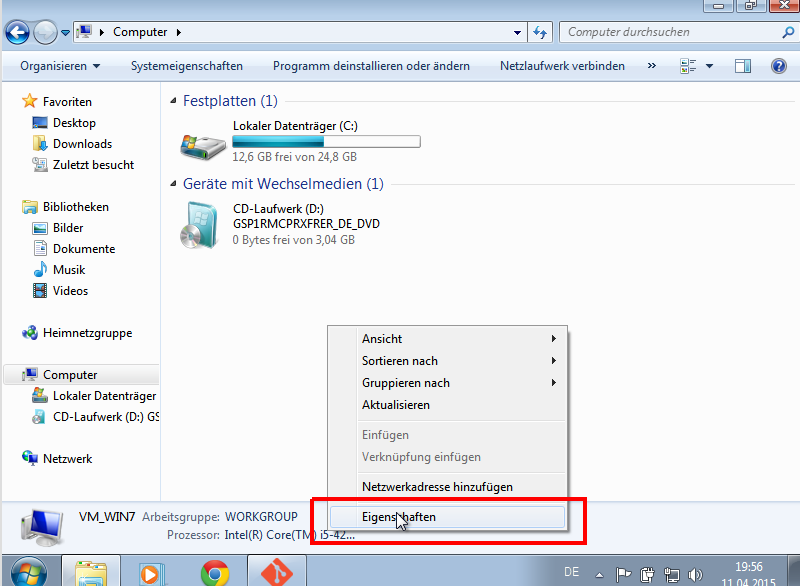
\includegraphics[width=.9\textwidth]{bilder/computer_properties}}
\end{center}

\clearpage
\noindent... öffnet sich ein neues Fenster. In diesem klickt man auf "Erweiterte Systemeinstellungen" ...

\begin{center}
	\makebox[\textwidth]{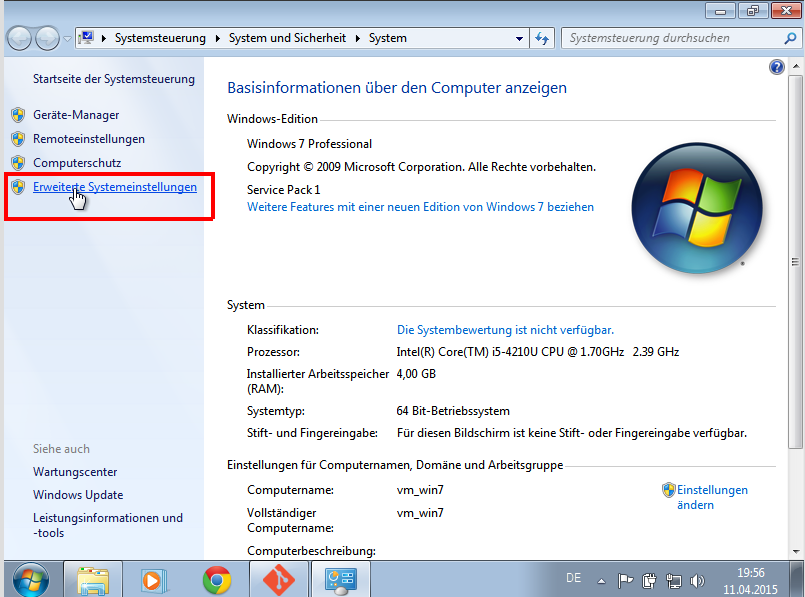
\includegraphics[width=.9\textwidth]{bilder/advanced_properties}}
\end{center}

\clearpage
\noindent... woraufhin sich ein Dialogfenster öffnet

\begin{center}
	\makebox[\textwidth]{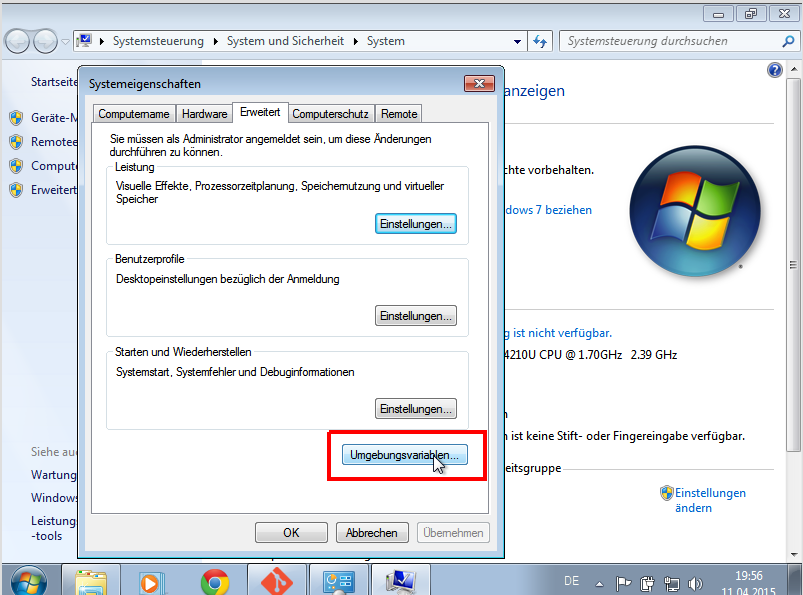
\includegraphics[width=.9\textwidth]{bilder/sys_vars}}
\end{center}

\clearpage


\subsection{Anpassen der Pfad-Umgebungsvariablen}

\textbf{Hinweis:} Es ist Vorsicht geboten beim Bearbeiten der Pfad-Variablen. Sollte diese aus Versehen gelöscht oder fehlerhaft bearbeitet werden, kann dies Auswirkungen auf andere Programme haben kann!
\\
\\
In dem Dialogfenster muss aus der Liste der Umgebungsvariablen die "Pfad"/"Path" ausgewählt werden.
Durch Klicken auf "Bearbeiten..." öffnet sich ein Dialog zum Bearbeiten der Pfad-Umgebungsvariablen.

\begin{center}
	\makebox[\textwidth]{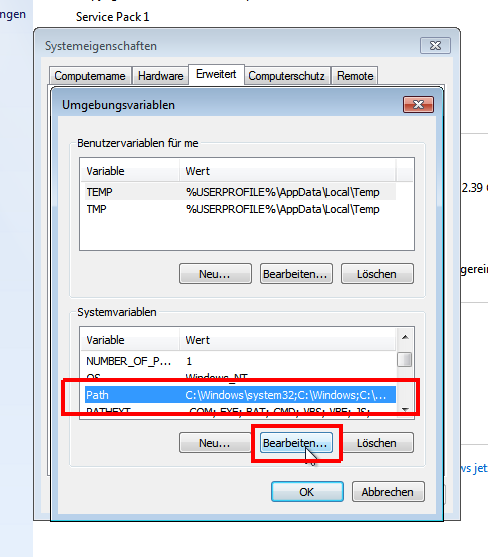
\includegraphics[width=.9\textwidth]{bilder/sys_vars_path}}
\end{center}

\begin{center}
	\makebox[\textwidth]{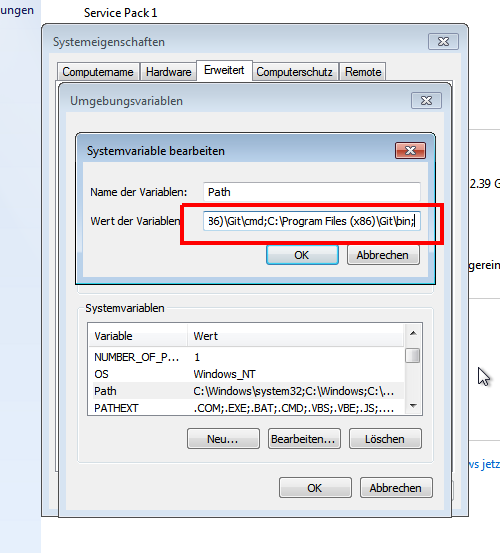
\includegraphics[width=.9\textwidth]{bilder/sys_var_path_edit_v1}}
\end{center}

\noindent Die Pfad-Umgebungsvariable ist eine Liste von Verzeichnispfaden, die mit ';' getrennt geschrieben sind.
\\
Nun muss am Ende mit ';' getrennt das Python-Installationsverzeichnis einfgefügt werden. Das Standardverzeichnis für Python 3.4 ist: C:\textbackslash Python34\textbackslash;.
\\
\\
\textbf{Hinweis:} Wurde der Pfad bei der Installation geändert, muss hier der geänderte Pfad eingetragen werden!
\\
\\
Zusätzlich muss auch noch das 'Scripts'-Verzeichnis im Python-Ordner, also C:\textbackslash Python34\textbackslash Scripts\textbackslash; zur Pfad-Variablen hinzugefügt werden. Dadurch können später weitere Python-Pakete mittels 'pip' installiert werden.
\\
\\
Insgesamt muss folgender Text (mit ggf. angepasstem Pfad) an das Ende angefügt werden:
\\

C:\textbackslash Python34\textbackslash;C:\textbackslash Python34\textbackslash Scripts\textbackslash;
\\

\begin{center}
	\makebox[\textwidth]{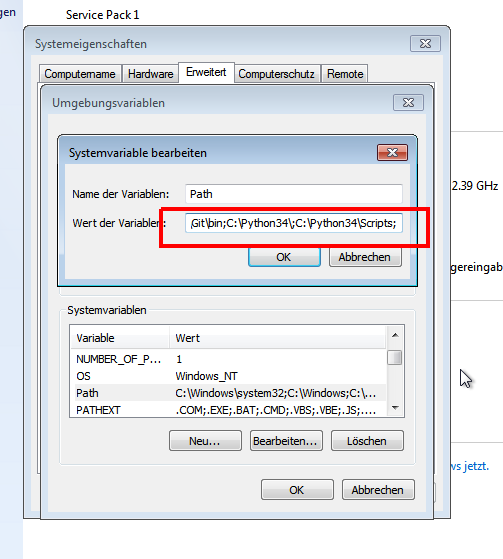
\includegraphics[width=.9\textwidth]{bilder/sys_var_path_edit_v2}}
\end{center}

\noindent Nach Bestätigung über "Ok" und Schließen der Fenster sollte die Pfadvariablen korrekt gesetzt sein.
\\
Dies kann wie in Schritt \ref{check_installation} beschrieben, überprüft werden.

\clearpage

\section{Editor}
Die Installation von Python sollte jetzt komplett sein. Nun ist nur noch die Frage zu klären, wie und mit welchem Programm Python programmiert werden kann.
\\
\subsection{IDLE}
Standartmäßig kommt mit Python die IDLE (Integrated Development Environment), die benutzt werden kann. Diese ist allerdings nicht allzu komfortabel zu benutzen, besitzt allerdings alle wesentlichen Funktionen. Die englische Dokumentation ist hier: \url{https://docs.python.org/3.4/library/idle.html} zu finden.
\begin{center}
	\makebox[\textwidth]{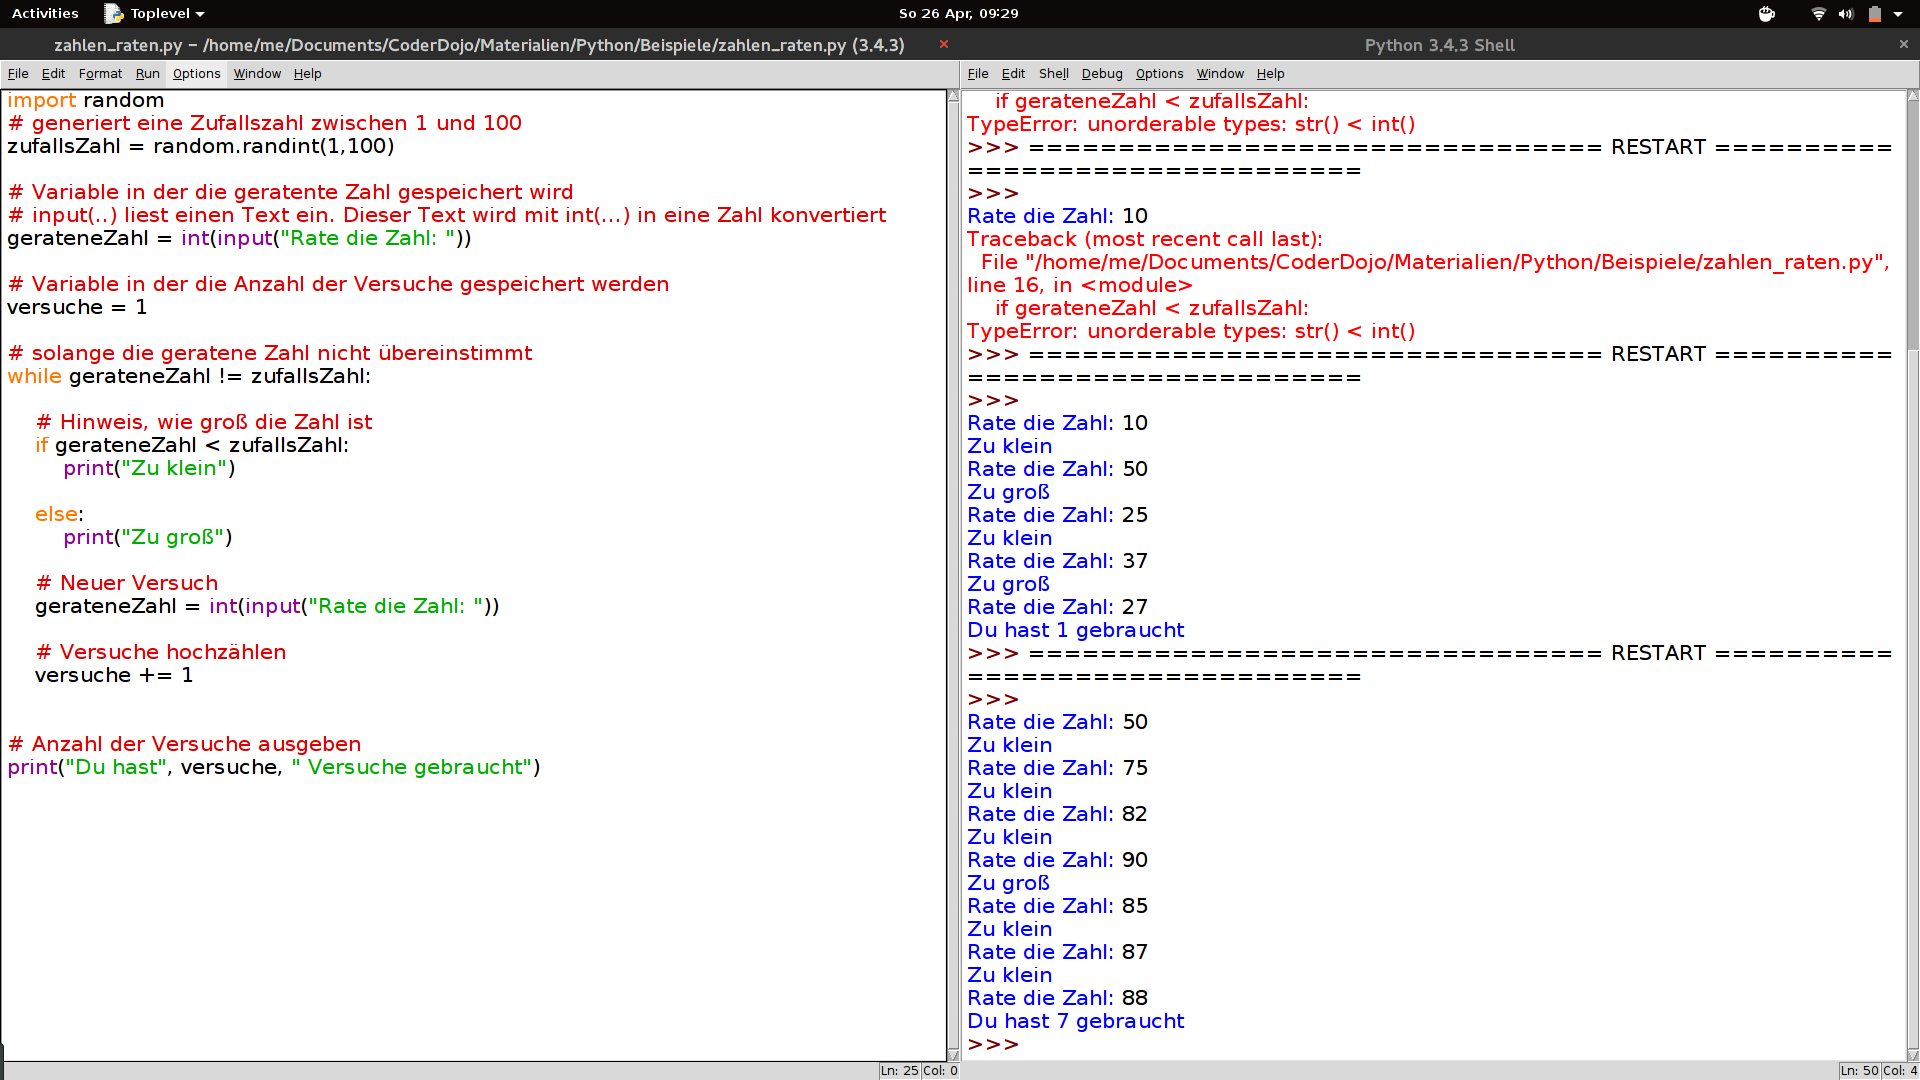
\includegraphics[width=.9\textwidth]{bilder/idle}}
\end{center}
Unter "File -\textgreater New" kann einen neue Datei erstellt werden. Unter "Run -\textgreater Run Module (F5)" kann die Datei ausgeführt werden. Dies öffnet ein "Python Shell Fenster". Es empfiehlt, solange der Bildschirm groß genug ist, beide Fenster nebeneinander zu haben.

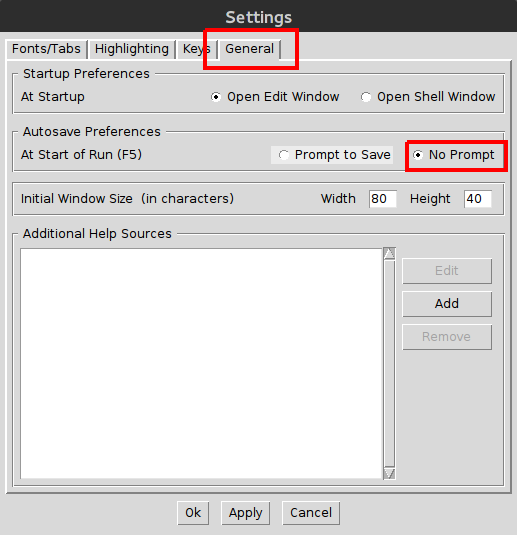
\includegraphics[width=100mm]{bilder/auto_save}
\\
Um die Datei auszuführen, ist es gut sich die Tastenkombination "F5" zum Ausführen zu merken und zu benutzen. Dafür ist es außerdem hilfreich, wenn man in den Einstellungen unter "Options -\textgreater Configure IDLE" im "General"-Tab die Einstellung bei "Autosave Preferences" auf "No Prompt" setzt, damit die Datei automatisch beim Ausführen gespeichert wird.

\end{document}
